\chapter{Rotation}
\graphicspath{{../../img/}}


In this lecture, we will discuss how to handle orientation. Robots are typically rigid bodies, that have position and orientation. Positions are simply $x,y, z$ coordinates but rotation is more complex. We will then discuss how we can model the motion and sensing of a robot and bring it back to the optimization theory we discussed. Hence, we have to be able to optimise over position and rotation.

We consider two frames - the world or the map $\{W\}$ and the body reference frame $\{B\}$, for the robot itself. Since the robot remains the same, we can specify the motion of one point $p(t) \in R^3$ and three coordinate axes $r_1(t), r_2(t), r_3(t)$, attached to that point.

\begin{figure}[h]\centering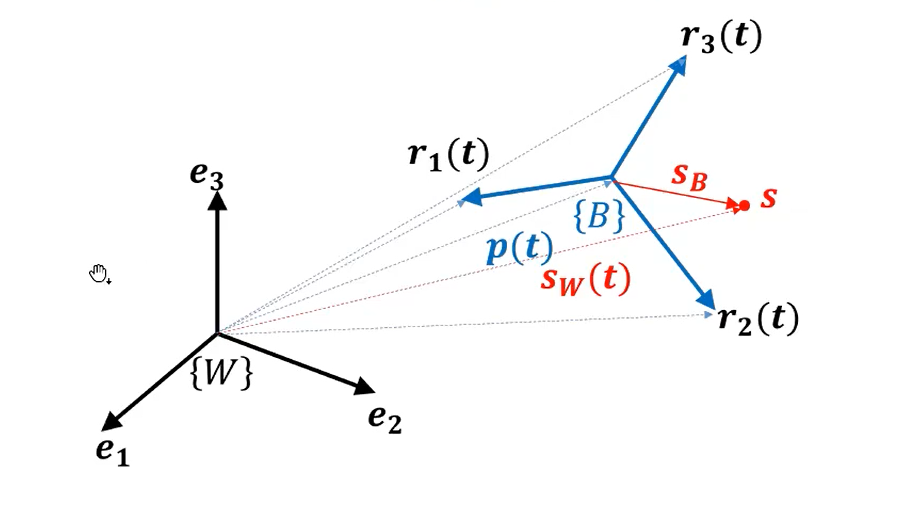
\includegraphics[width=12cm]{img/j_1.png}\end{figure}

In the above figure, we can see the black axes as the world frame, and the blue lines as the body frame. The point $s$ will have constant coordinates with respect to the body frame (it is some point on the robot), but different coordinates in the world frame (since the body is constantly moving). Alternatively,

A point $s$ on the rigid body has fixed coordinates $s_B\in R^3$ in the body frame $\{B\}$ but time-varying coordinates $s_w(t)\in R^3$ in $\{W\}$.

\textbf{Pose}

The pose $T(t)\in SE(3)$ of a rigid body reference frame $\{B\}$ at time $t$ in a fixed world frame $\{W\}$ is determined by:

\begin{enumerate}
    \item The position $p(t)\in R^3$ of $\{B\}$ relative to $\{W\}$.
    \item The orientiation $R(t) \in SO(3)$ of $\frame{B}$ relative to $\frame{W}$, determined by the 3 coordinate axes $r_1(t), r_2(t), r_3(t)$.
\end{enumerate}

Now, how do we describe the space of orientations of orientations $SO(3)$ and the space of poses $SE(3)$.

\section{Special Euclidian Group}

Rigid body motion is described by a sequence of functions that describe how the coordinates of 3-D points on the object change with time.

Rigid body motion preserves distances (vector norms) and does not allow reflection of the coordinate system (vector cross products).

For instance, the distance between our eyes should not change when we move around. Further, it shouldn't be possible to get a mirror image of a body when it moves.

The \textbf{Euclidian Group} $E(3)$ is a set of functions $g: R^3\to R^3$ that preserves the norm of any two vectors.

The \textbf{Special Euclidian Group} $SE(3)$ is a set of functions $g: R^3\to R^3$ that preserve the norm and the cross product of any two vectors.

\begin{enumerate}
    \item Norm: $\norm{g_*(u) - g_*(v)} = \norm{v-u}, \forall u, v \in R^3$.
    \item Cross product: $g_*(u) \times g_*(v) = g_*(u\times v), \forall u, v \in R^3$
\end{enumerate}

where $g_*(x) := g(x) - g(0)$.

\textbf{Corollary:} $SE(3)$ elements $g$ also preserve:

\begin{enumerate}
    \item Angle: $u^Tv = \frac{1}{4} (\norm{u + v}^2 - \norm{u-v}^2) \implies u^Tv = g_*(u)^T g_*(v), \forall u, v \in R^3$.
    \item Volume: $\forall u, v, w \in R^3, g_*(u)^T(g_*(v)\times g_*(w))=u^T(v\times w)$
\end{enumerate}

\section{Rotation}

Pure rotation is a special case of rigid body motion. The orientation of the body frame $\frame{B}$ in the world frame $\frame{W}$ is determined by the coordinates of the three orthogonal vectors $r_1 = g(e_1), r_2 = g(e_2), r_3 = g(e_3)$, transformed from $\frame{B}$ to $\frame{W}$.

The vectors organized in a $3\times 3$ matrix specify the orientation of $\frame{B}$ in $\frame{W}$:

\begin{equation*}
    {}_{\frame{W}}R_{\frame{B}} = \begin{bmatrix}
        r_1 & r_2 & r_3
    \end{bmatrix} \in R^{3\times 3}
\end{equation*}

Consider a point with coordinates $s_B\in R^3$ in $\frame{B}$. Its coordiantes $s_W$ in $\frame{W}$ are:

\begin{equation*}
    \begin{split}
        s_W &= [s_B]_1r_1 + [s_B]_2r_2 + [s_B]_3r_3 \\
        &= Rs_B
    \end{split}
\end{equation*}

\begin{figure}[h]\centering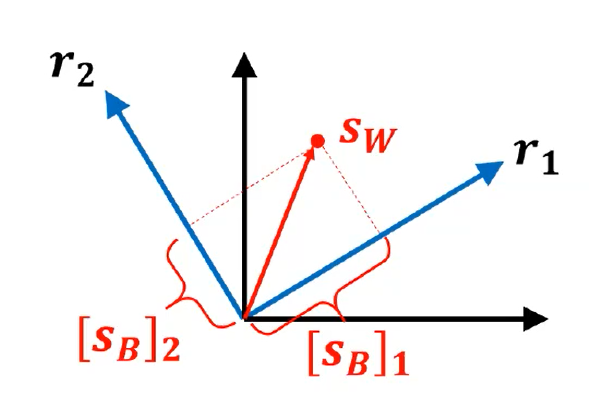
\includegraphics[width=7cm]{img/j_3_2.png}\end{figure}

The rotation transformation $g$ from $\frame{B}$ to $\frame{W}$ is:

\begin{equation*}
    g(s) = Rs
\end{equation*}

\section{Special Orthogonal Group $SO(3)$}

$r_1, r_2, r_3$ from an orthonormal basis: $r_i^Tr_j = 1$ (when $i=j$), else $0$.

Since $r_1, r_2, r_3$ form an orthonormal basis, the inverse of R is its transpose $R^TR=I$ and $R^{-1} = R^T$.

\begin{figure}[h]\centering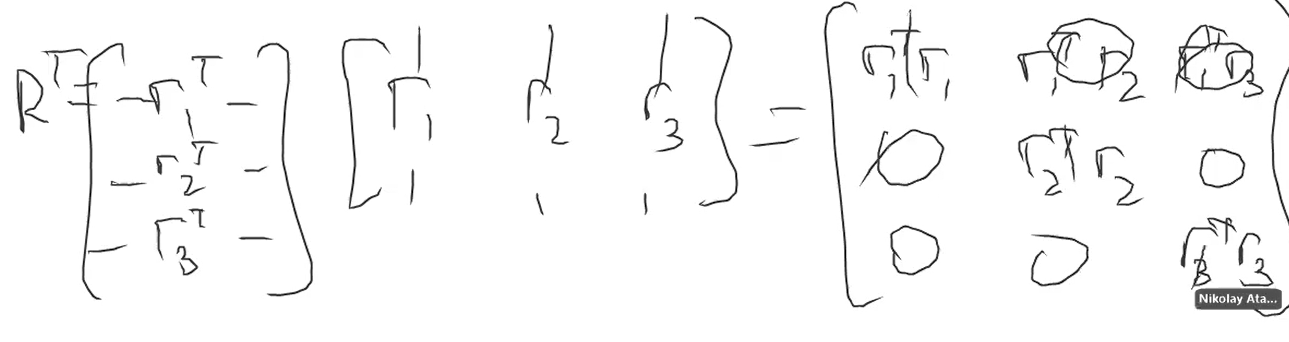
\includegraphics[width=12cm]{img/j_3_3.png}\caption{A quick illustration to see why $R^TR=I$}\end{figure}

$R$ belongs to the orthogonal group:

\begin{equation*}
    O(3): = \{ R\in R^{3\times 3} | R^TR = RR^T = I\}
\end{equation*}

Distance preserving: Let's look at -

\begin{equation*}
    \begin{split}
        \norm{Rx - Ry}_2 = \norm{R(x - y)}^2 = (x - y)^TR^TR(x - y) = (x - y)^T(x - y) = \norm{x - y}^2
    \end{split}
\end{equation*}


Reflections are not allowed since $\text{det}(R) = r_1^T(r_2\times r_3) = 1$:

\begin{equation*}
    R(x\times y) = R(x\times (R^TRy)) = (R\hat{x}R^T)Ry = \frac{1}{det(R)}(Rx)\times (Ry)
\end{equation*}

Hence, we can say that $R$ belongs to the special orthogonal group:

\begin{equation*}
    SO(3) : = \{ R\in R^{3\times 3} | R^TR = I, det(R) = 1\}
\end{equation*}
